\documentclass[a4paper,12pt]{article}

% Pacotes básicos
\usepackage[utf8]{inputenc}
\usepackage[T1]{fontenc}
\usepackage[portuguese]{babel}
\usepackage{amsmath, amssymb, amsfonts, mathtools} % Para matemática
\usepackage{graphicx} % Para incluir imagens
\usepackage{listings} % Para blocos de código
\usepackage{xcolor} % Cores
\usepackage[colorlinks=true, linkcolor=black, urlcolor=black, citecolor=black]{hyperref} % Links no documento
\usepackage{geometry} % Configuração de margens
\usepackage{titlesec}
\usepackage{ragged2e} % Para \justifying


% Configurar títulos de seções e subseções à esquerda
\titleformat{\section}[hang]{\bfseries\Large\raggedright}{\thesection}{1em}{}
\titleformat{\subsection}[hang]{\bfseries\large\raggedright}{\thesubsection}{1em}{}

\usepackage[perpage]{footmisc}
\usepackage{indentfirst} % Recuo de parágrafo
%\usepackage{times} % Fonte Times New Roman pq o Henrique quis


% PACOTE DE CITAÇÕES
\usepackage[style=abnt,backend=biber]{biblatex} % Usa biblatex para citações e referências
\addbibresource{references.bib} % Nome do arquivo .bib


% Configurações ais
\geometry{a4paper,margin=2.5cm}


\makeatletter
\let\@fnsymbol\@arabic
\makeatother

\setlength{\parskip}{.5em} % Espaçamento entre parágrafos de 1em

% Configurações do título
\title{Relatório do trabalho de Linguagens da Programação}
\author{
        Davi de França Vasconcelos Nunes
        \footnote{FGV - Rio de Janeiro/RJ  - Ciência de Dados e Inteligência Artificial - Matrícula: 241708053} \\
        Henrique Gabriel Gasparelo 
        \footnote{FGV - Rio de Janeiro/RJ - Ciência de Dados e              Inteligência Artificial - Matrícula: 241708055} \\
        Isaías Gouvêa Gonçalves
        \footnote{FGV - Rio de Janeiro/RJ - Ciência de Dados e Inteligência Artificial - Matrícula: 241708012} \\
        José Thevez Gomes Guedes
        \footnote{FGV - Rio de Janeiro/RJ - Ciência de Dados e Inteligência Artificial - Matrícula: 241708005} \\
        } 
\date{\today}

%%%%%%%%%%%%%%%%%%%%%%%%%%%%%%%%%%%%%%%%%%%%%%%%%%%%%%%%%%%%%%%%%%%%%%%%%%%%
% Início do documento%%%%%%%%%%%%%%%%%%%%%%%%%%%%%%%%%%%%%%%%%%%%%%%%%%%%%%%
\begin{document}

% Título
\maketitle
\vspace{-1cm}

% Sumário
\tableofcontents

\newpage

%INTRODUÇÃO%%%%%%%%%%%%%%%%%%%%%%%%%%%%%%%%%%%%%%%%%%%%%%%%%%%%%%%%%%%%%%%%%
\section{Introdução} 

Neste trabalho foi elaborado um jogo de aventura, ação e RPG, utilizando a linguagem \textit{Python} e a biblioteca \textit{Pygame}. Nomeado "Atwo Survivors", foi inspirado no conceito de \textit{Vampire Survivors}, a partir do qual recebeu suas modificações na mecânica de jogo e funcionalidades. O presente relatório visa apresentar como o jogo foi elaborado, com a divisão das tarefas do grupo, principais características do processo de desenvolvimento e dificuldades observadas.


\section{Apresentação do Jogo}

O Atwo Survivors se inspirou nas mecânicas principais do jogo Vampire Survivors, consistindo em um jogo de visão periférica (semelhante aos jogos de RPG tradicionais) em que um personagem principal deve combater diversos inimigos que aparecem de forma aleatória no mapa e sobreviver, até que, após um certo intervalo de tempo, o jogador deve enfrentar um \textit{boss}. Na versão apresentada do jogo, o personagem principal deve vencer dois \textit{bosses} para vencer. Ao longo do jogo, ao combater inimigos, o jogador coleta pontos de experiência, que evoluem seu nível e o permitem aprimorar suas habilidades, adquirir novas armas e evoluí-las.

\begin{figure}[h!]
    \centering
    \caption{Captura de tela de Atwo Survivors}
    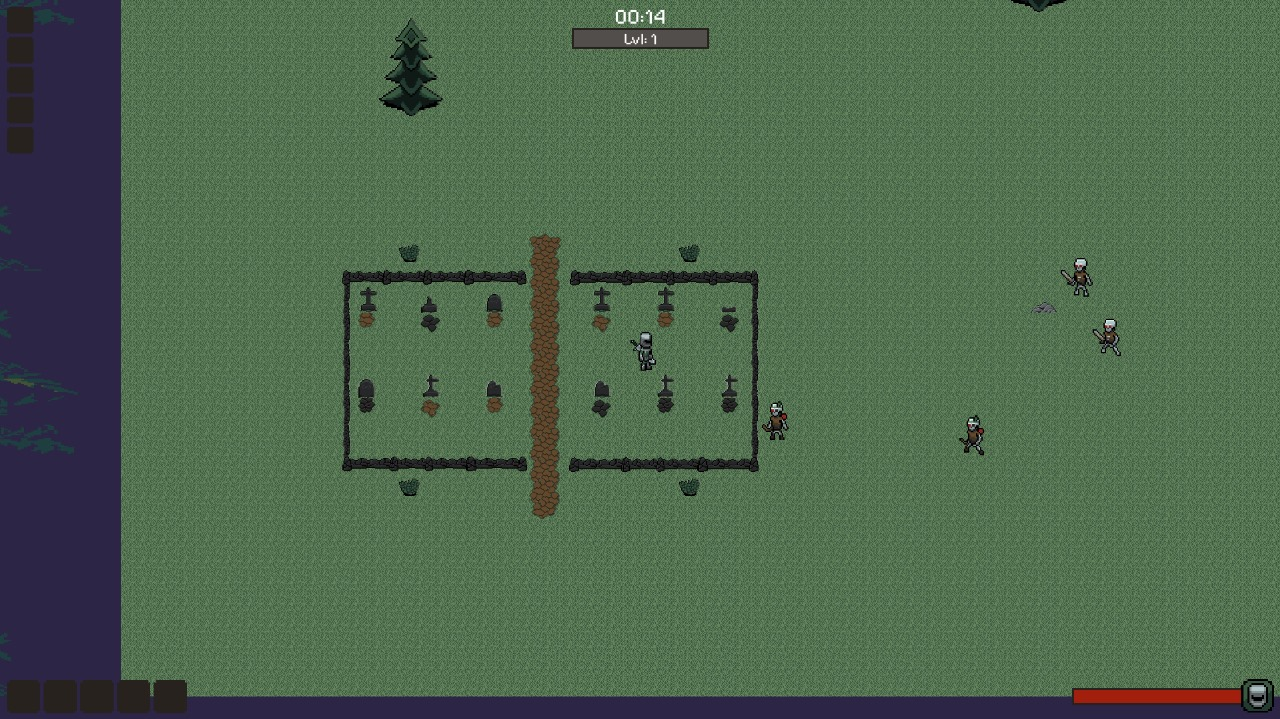
\includegraphics[width=0.7\linewidth]{imgs/gp1.jpeg}\\
    {Fonte: Autoria própria}
\end{figure}

A diferença central entre o Atwo Survivors e o jogo no qual se inspirou é a mecânica de combate: originalmente o ataque é automático, onde o jogador controla somente os movimentos do personagem e gerencia suas habilidades. No Atwo Survivors, o jogador também é responsável pelos ataques a serem utilizados, selecionando a arma a ser utilizada e em que momento e direção serão feitos os ataques. Tal recurso aumenta consideravelmente a dificuldade do jogo.


%%%%%%%%%%%%%%%%%%%%%%%%%%%%%%%%%%%%%%%%%%%%%%%%%%%%
\section{Escolhas de Design}

A princípio o jogo possui uma temática medieval, uma vez que o personagem principal utiliza uma armadura. Da mesma forma, as primeiras criaturas e os cenários reforçam essa primeira impressão. No entanto, ao decorrer do jogo, a presença de alguns itens como uma escopeta e o segundo \textit{boss} revelam a escolha de design inusitada que foi adotada para o Atwo Survivors, que mistura elementos medievais com outros de diferentes temáticas. O jogador poderá lidar com ataques mágicos, armas de fogo ou uma simples espada.

\begin{figure}[h!]
    \centering
    \caption{Captura de tela de Atwo Survivors}
    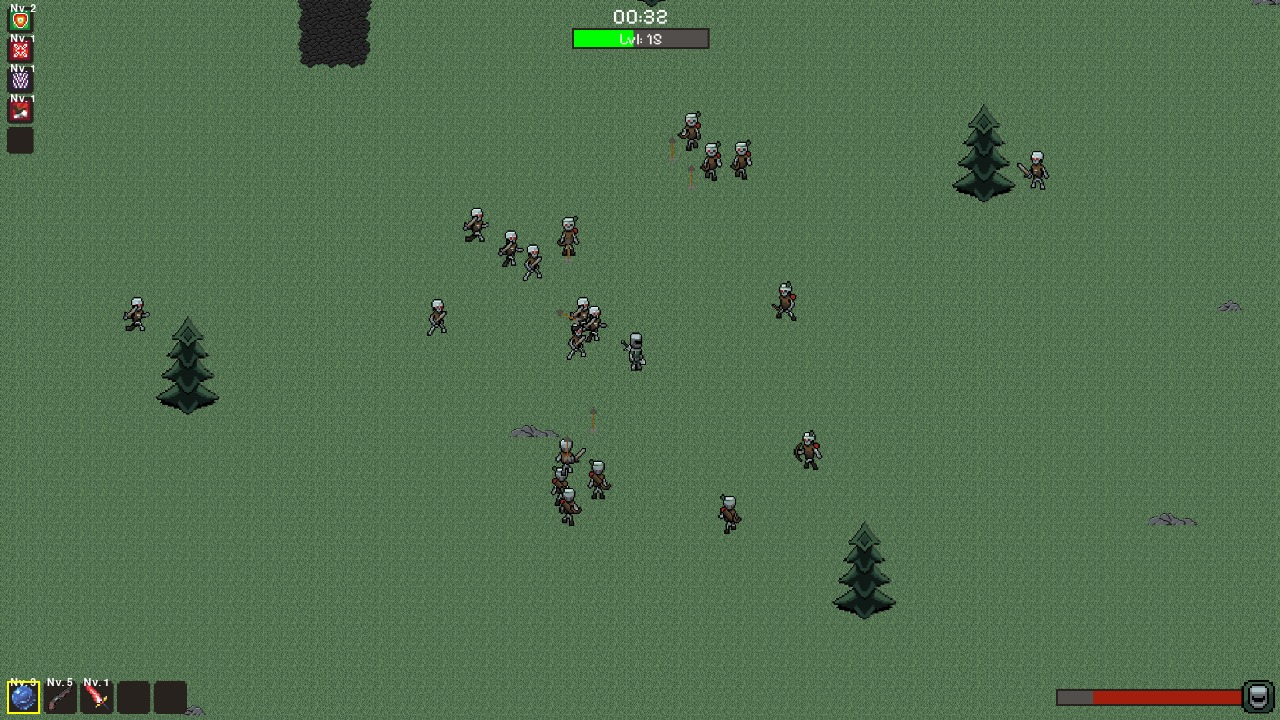
\includegraphics[width=0.7\linewidth]{imgs/gp2.jpeg}\\
    {Fonte: Autoria própria}
\end{figure}

Os \textit{sprites} principais\footnote{Os demais sprites podem ser encontrados em \href{https://c1aymor3.itch.io/basic-gun-asset-pack}{https://c1aymor3.itch.io/basic-gun-asset-pack} e \href{https://pixelcreations.itch.io/rpg-items-16x16}{https://pixelcreations.itch.io/rpg-items-16x16}} do jogo foram obtidos na plataforma \textit{Itch.io} e produzidos pelo artista Foozle\footnote{Os arquivos podem ser encontrados no pacote "Lucifer" \space disponível em: \href{https://foozlecc.itch.io/}{https://foozlecc.itch.io/}}. 

A sonoplastia do jogo foi elaborada a partir de efeitos sonoros gratuitos de uso livre, e a trilha sonora foi criada com inteligência artificial. 

\begin{figure}[h!]
    \centering
    \caption{Menu inicial de Atwo Survivors}
    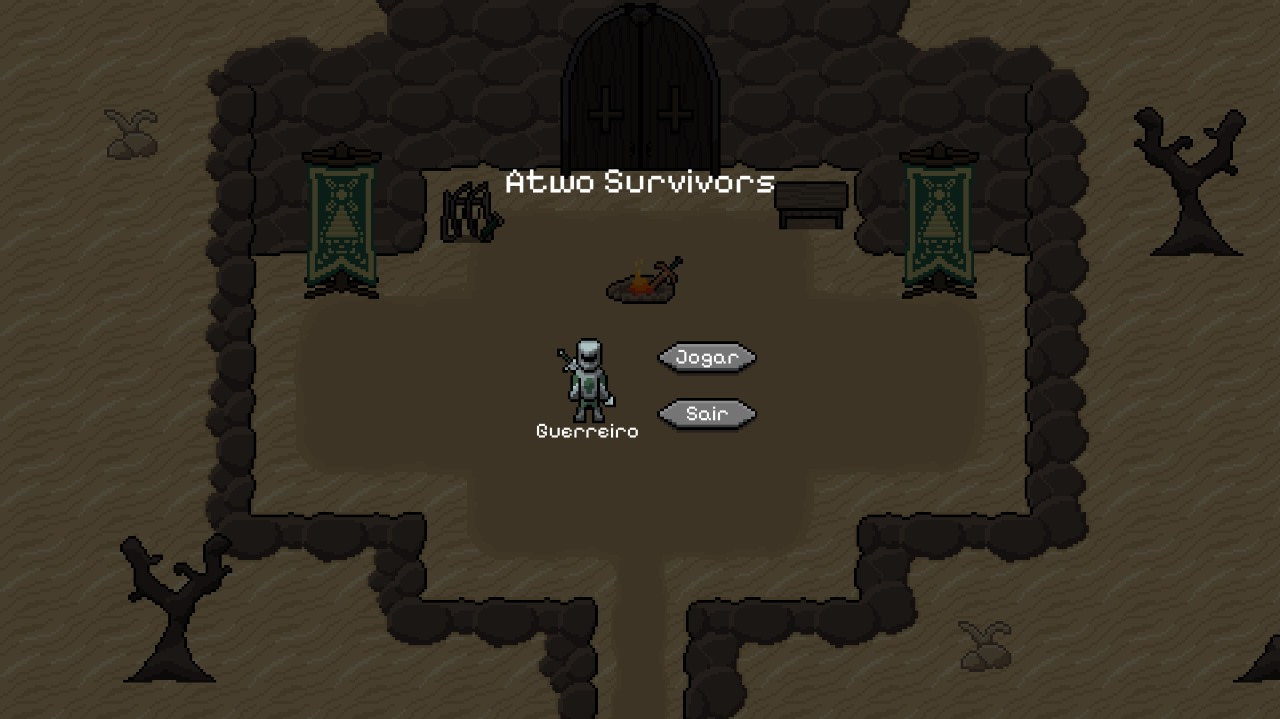
\includegraphics[width=0.7\linewidth]{imgs/menu.jpeg}\\
    {Fonte: Autoria própria}
\end{figure}

\newpage



\section{Processo de desenvolvimento}

O jogo foi desenvolvido sob a lógica de orientação a objetos, em que o código fonte esteve subdividido em arquivos que contêm as classes e seus respectivos métodos, implementando as funcionalidades do jogo. A pasta \texttt{/src} está organizada nos seguintes módulos:

\begin{itemize}
    \item \texttt{main.py}: Inicia o loop principal do jogo.
    \item \texttt{config.py}: Configurações do jogo (ex.: parâmetros do jogo).
    \item \texttt{drop\_item.py}: Lógica relacionada à drop de itens.
    \item \texttt{enemies.py}: Definições e propriedades das classes de inimigos.
    \item \texttt{enemy\_ai.py}: Inteligência artificial dos inimigos.
    \item \texttt{game.py}: Lógica principal do jogo e inicialização.
    \item \texttt{items\_abilities.py}: Gerenciamento de itens e habilidades do jogo.
    \item \texttt{main\_character.py}: Código para o personagem do jogador (ex.: movimento, interações).
    \item \texttt{map.py}: Gerenciamento de mapas e tiles.
    \item \texttt{props.py}: Manipulação de objetos interativos no ambiente do jogo.
    \item \texttt{repositorio\_sons.py}: Gerenciamento de recursos de áudio e reprodução de sons.
    \item \texttt{repositorio\_sprites.py}: Carregamento e gerenciamento de recursos de sprite.
    \item \texttt{sprites.py}: Manipulação e renderização de sprites.
    \item \texttt{ui.py}: Componentes da interface do usuário e renderização.
\end{itemize}


\section{Dificuldades encontradas}

Apesar de ser uma biblioteca por si só repleta de funcionalidades, o \textit{Pygame} ainda assim é significativamente mais difícil de se trabalhar do que uma \textit{game engine} mais popular, como \textit{Unity}, \textit{Unreal} ou \textit{RPG Maker}, uma vez que as principais funcionalidades do jogo, como movimento, animação, dano, dentre outros, devem ser feitas de forma "crua" \space no código, sem a utilização de \textit{frameworks} prontas e adaptadas à necessidade do desenvolvedor. Desta forma, diversas dificuldades foram encontradas no processo de criação do jogo.

\paragraph{Movimentação dos inimigos:} Os inimigos do jogo devem atacar o personagem principal, e para isso deve existir um sistema de movimentação que leve o inimigo até o personagem em uma velocidade consistente. Não existe nenhum recurso nativo de Pygame que permite essa movimentação. 

A solução adotada, portanto, utiliza um pouco de álgebra linear: é traçado um vetor entre o inimigo e o jogador, esse vetor é então normalizado (tem sua distância encurtada para um, para conter apenas a informação da direção do deslocamento) e depois é inserida na movimentação do inimigo a partir da velocidade padrão. A mesma estratégia foi usada para os \textit{bosses}, com pequenas alterações.

\paragraph{\textit{Spawn} de itens e inimigos:} Para que haja uma dinâmica de jogo, ao logo do mapa devem ser gerados itens coletáveis e inimigos a serem combatidos. Uma mecânica que poderia em primeira instância parecer fácil gerou diversas dificuldades ao longo do desenvolvimento, especialmente por conta de diversos \textit{bugs} que foram corrigidos das mais diferentes formas de acordo com a necessidade.

\paragraph{Ataque à distância:} Assim como a perseguição de inimigos, o ataque à distância foi mais um grande desafio utilizando vetores. No entanto, esse em particular apresenta uma dificuldade a mais: manter a renderização de um ataque em curso desconsiderando possíveis movimentações da câmera do jogo. A solução foi feita por meio de adaptações nas coordenadas atualizadas em tempo real. 

\section{Divisão dos trabalhos}

Naturalmente, em um trabalho de dimensões como esse, as tarefas tiveram de ser divididas entre os membros do grupo para que o projeto saísse conforme esperado. As divisões não foram seguidas perfeitamente à risca pois diferentes demandas surgiram ao longo do desenvolvimento, além de que em certos momentos do projeto, nem todos os membros puderam se dedicar integralmente. A divisão fundamental das tarefas ficou da seguinte forma:

\begin{itemize}
    \item \textbf{Henrique Gasparelo:} Interface de usuário, Arquivo principal do jogo, correção de \textit{bugs}, sonoplastia, design.
    \item \textbf{José Thevez:} Personagem principal, movimentação, mecânicas de combate, inimigos, mecânicas dos \textit{bosses}, sonoplastia, mecânicas de animação.
    \item \textbf{Davi França:} Cenário do jogo, \textit{spawn} de itens coletáveis no mapa.
    \item \textbf{Isaías Gonçalves:} Inimigos, animações, sistema de inteligência artificial de perseguição, relatório.
\end{itemize} 


% \begin{figure}[h!]
%     \centering
%     \caption{Gráfico antigo da primeira hipótese.}
%     \includegraphics[width=0.7\linewidth]{images//hip_1/hip_1_antigo.png}\\
%     {Fonte: Autoria própria}
%     \label{fig:1}
% \end{figure}


\section{Considerações Finais}

Neste trabalho foi desenvolvido o jogo Atwo Survivors, construído a partir de um código em branco em que foram explorados os mais diversos recursos da biblioteca Pygame. A experiência de desenvolvimento foi desafiadora, e oportunidade para diversos aprendizados sobre a rotina de desenvolvimento de um projeto mais aprofundado. O resultado final supriu as expectativas de um jogo com todas as principais mecânicas e dinâmicas de progressão, sendo portanto um projeto satisfatório. 


% Referências
%\printbibliography

% Apêndice%%%%%%%%%%%%%%%%%%%%%%%%%%%%%%%%%%%%%%%%%%%%%%%%%%%%%%%%%%%%%%%%%%

\end{document}
